%%%%%%%%%%%%%%%%%%%%%%%%%%%%%%%%%%%%%%%%%%%%%%
\logvartrue
\chapter{Background}
%%%%%%%%%%%%%%%%%%%%%%%%%%%%%%%%%%%%%%%%%%%%%%

Bacteria are often cited as examples of one of the Earth's most primitive living forms. Unfortunately, they are still associated almost exclusively to infection diseases. The reality is rather different, in fact only a very small fraction of bacteria is able to cause infections in contrast to a highly diversified and beneficial bacterial world. Most of them not only reciprocally support each other but their immensely varied and efficient metabolism also defines and sustains balanced environments (the biosphere). Solidarity among bacterial cells is one of their most important characteristic. Even infection-causing bacteria are able to benefit from this solidarity, making them more resilient and ``inventive'' than isolated species. In the last 20 years, the development of genomic tools have revolutionized microbial ecological studies and strongly expanded our view on this previously under appreciated microbial world. It is encouraging to see that evolution and ecology are now emerging as regular subjects within microbiology. The next decade should be one of gradually changing and enlarging perspective regarding the place of bacteriology in the biological sciences. There are now comforting signs that we are moving towards a deeper and more realistic appreciation of the roles played by bacteria on our planet.

\section{The Bacterial world}
Microorganisms are essentially everywhere in nature and they have been integral to the history and function of life on Earth. However, until very recently, their importance has been appreciated by only a few specialist. Indeed, bacteria are still most often considered from an anthropocentric point of view, focusing our attention only on the relatively few pathological species and the potential of microorganisms to provide us with useful products and services (\textbf{da mettere un paio di references}). This is a very constrained perspective if we think that bacteria have been the sole form of life on Earth for some two billion years, playing central roles in climatic, geological, geochemical, and biological evolution \cite{cavalier2006cell}.\\
The bacterial world contains a highly heterogeneous group of organisms sharing only one common characteristic, their small size. The patterns of bacteria distribution are influenced by environmental factors such as temperature, pH, salinity, pressure, the presence of nutrients and the sources of carbon and energy \citep{gerhard1986bacterial}. These factors are able to shape Earth's bacterial communities distribution in respect to both space and time, influencing the selective proliferation of a set of bacteria in a distinct environment, based on their metabolic characteristics. Bacteria can use many different types of metabolic strategies and bacterial species can often be differentiated from each other based on their metabolic characteristics. The specific metabolic properties of a microbe are one of the major factors in determining that microbe’s ecological niche, and they can be used to classify bacteria in different metabolic groups (Figure~\ref{fig:bacmet}). Thanks to their high variability, bacteria have been, and still are able to colonize almost every ecological niche in nature.\\
\begin{figure}[!tb]
	\centering
	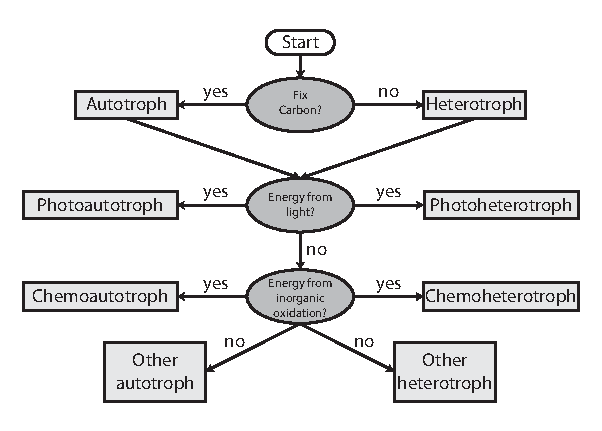
\includegraphics[width=0.7\textwidth]{./figures/Introduction/bacterial_metabolism_bw}
  	\caption{General flowchart used for metabolic classification of bacteria. \label{fig:bacmet}}
\end{figure}
Giving their ability to thrive in a vast set of different environments, bacteria play pivotal roles in several biogeochemical cycles and are responsible for the cycling of organic compounds. They have been found in all kind of environments ranging from the human gut \cite{walter2011human}, to the rhizosphere \cite{philippot2013going}, to conventionally inhospitable habitats such as acid mine run-off \cite{simmons2008population} and geothermal hot springs 	\cite{sharp2014humboldt}. Studies based on cultured microbes have revealed that they are critical components of these environments providing them with essential services \cite{van2008unseen, arrigo2004marine}. For example, the Earth's cycles of hydrogen, carbon, nitrogen, oxygen and sulphur are driven largely by microbial catalysed redox reactions (Figure \ref{}). These reactions require multimeric protein complexes evolved exclusively in microorganism such as bacteria \cite{falkowski2008microbial}. However, a large part of these processes is still unknown making the study of bacterial functions indispensable for the complete comprehension of the dynamics able to modify our planet.\\
Biologists have long appreciated the roles that microbes play in the two distinct disciplines of pathogenesis and ecosystem cycling; although, in these years, the importance of microbes-host association is rapidly growing. Currently, microbes associated with a macroscopic host have their own definition in the word ``microbiota'' coined for the firs time by Joshua Lederberg in 2001 \citep{lederberg2001scientist}. The role of microbiota is occupying a very important position in the host evolution \cite{ley2008evolution}. Indeed, the set of bacteria linked with a macroscopic organism can interact with its host to influence physiology and contribute to health, growth, or fitness \citep{dimkpa2009plant, hooper2012interactions}. For example, studies of model rhizosphere microbiota have taught us that they can impact plant growth \citep{kennedy2007competitive}, stress response \cite{redman2002thermotolerance, yang2009rhizosphere}, and pathogenic defense \cite{cook1995molecular}. In this perspective, for understanding completely a macroscopic organism’s physiology is becoming mandatory the investigation of its microbiota.\\
This great microbial diversity found in various environments (including hosts associated ones) can be measured by a set of indices such as phylogenetic diversity, species diversity, genotype diversity, and gene diversity. Above the species level, microbial diversity has been commonly quantified based on evolutionary distances among observed taxonomic groups from a specific environment. Below this level, microbial diversity has been typically described using population genetic parameters such as gene diversity and genotype diversity. However, despite the fact that species is the fundamental unit of biological classification, what constitute a species remain controversial. In addition, until very recently, most of what we know about microbial diversity and microbial functions were derived from cultured microorganisms . While such studies are essential, the advent of genomic has revolutionized our comprehension of the bacterial world showing that much of what we thought we knew about this microscopic world were in fact highly biased.\\

\subsection{The species concept}
%\begin{wrapfigure}{r}{0.35\textwidth}
%	\vspace{-20pt}
%	\begin{center}
%		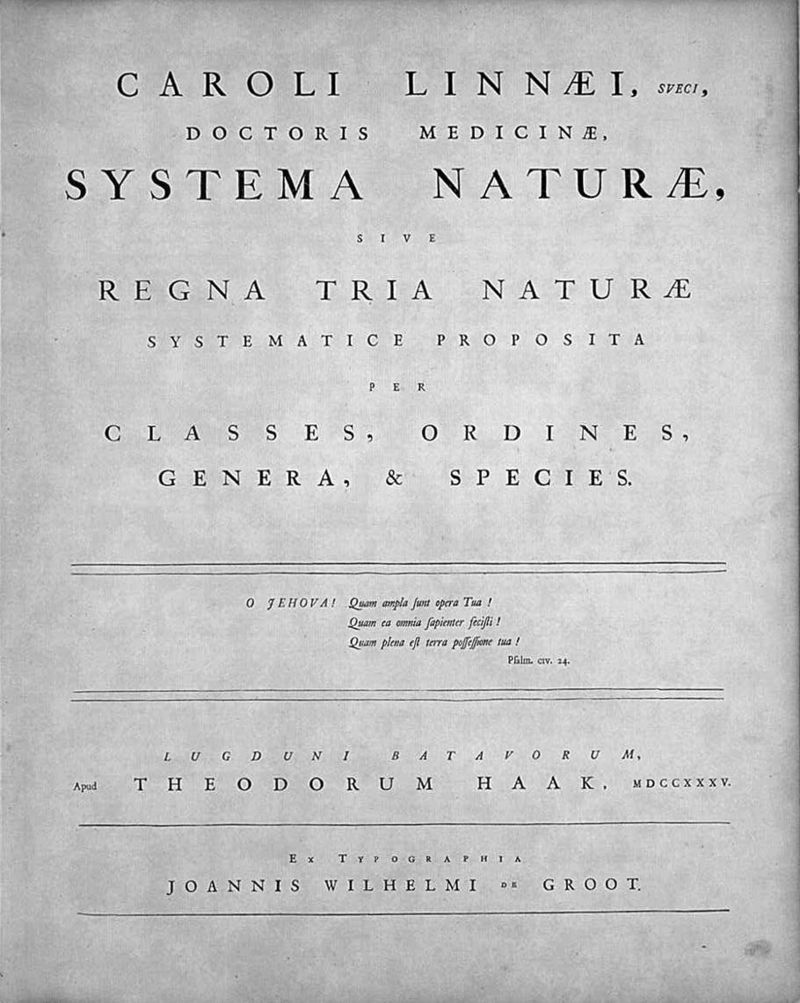
\includegraphics[width=0.33\textwidth]{./figures/Introduction/systema_naturae}
%	\end{center}
%	\caption{The title page of Systema Naturae, Leiden (1735)}
%	\vspace{-10pt}
%\end{wrapfigure}
Attempting to bring order in the astounding variety of organisms with which we share the planet have been an endless human effort. One of the first classification system was developed by Carl Linnaeus in the mid-18th century \cite{linnaeus1800species, bhl10277}. Linnaeus established the existence of three kingdoms: the animal kingdom (\textit{Regnum animale}), the plant kingdom (\textit{Regnum vegetabile}) and the mineral kingdom (\textit{Regnum lapideum}), outlining his ideas for the hierarchical classification of the natural world. In his works Linnaeus did not classify microbes but, since the mid-19th century, his binomial nomenclature has been used by microbiologist to designate microbial species. However, what constitute a species was and remains  controversial especially with the advent of the ``genomic era'' and the explosion of data that it has brought with it \cite{doolittle2006genomics}.\\
Prokaryotic classification is the youngest and most dynamic between all classifications of living organisms. This might be due to the fact that prokaryotes were not even know to exist until a few centuries ago. Developing a prokaryote classification system based on macro-morphological traits, like sexual reproduction or some physical characteristics, has been a very difficult because of their relative simplicity \cite{cowan1965principles}. The absence of useful fossil records, together with the difficulties in identifying possible diagnostic elements from these organisms have concur to the instability of the prokaryote classification system. Indeed, species demarcation in prokaryotes is not defined by a theory-based concept and tends to be more arbitrary, anthropocentric or rooted in practical necessity (e.g. bacteria species like \textit{Neisseria meningitis} or \textit{Bacillus anthracis} have been historically defined on the basis of the disease they cause regardless of other types of considerations).\\
Until the end of the 18th century, no prokaryotic classification was attempted. Ottu M\"{u}ller, a Danish naturalist, was the first to create a systemic arrangement of microorganisms defining two form genera called \textit{Vibrio} and \textit{Monas}; which differentiated the round and elongated type of bacterial cells \cite{logan2009bacterial}. One of the most important step in the classification of microorganisms was the ability to isolate them in pure cultures. Therefore, in 1881, Robert Koch published the first technique of cultivation on a solid media; paving the way for what he called ``the golden age of the medical microbiology''. Following this discovery, researchers were able to retrieve direct informations on a microorganism by cultivating it in pure culture; thus, the amount of bacteria described from the end of the 19th century to the first two decades of the 20th century was impressive. In 1970  a modern identification index for bacteria was first provided with the publication of the ``Bergey's Manual of Determinative Bacteriology''. In the second half of the 20th century the increasing knowledge of the properties DNA, in conjunction with the development of molecular biological techniques pushing the idea that bacteria might be classified using their genomes. Finally, in 1970, the catalogation of the ribosomal RNA (rRNA) and the development of the DNA-DNA hybridization technique permitted to achieve a great breakthrough in the history of bacterial classification \cite{stackebrandt198516, de1975improvements}.\\
Currently, microbial species are defined using the so-called "polyphasic approach", that is grounded on clear rules for both genotypic and phenotypic attributes \cite{vandamme1996polyphasic}. Nowadays, more than 7000 different microbial species have been classified using this approach, but, as actually practised, it faces serious problems. Indeed, the primary criterion for discriminating between different species is a cut-off level for pairwise genomic DNA-DNA hybridization levels; however, this cut-off level has never been based on any particular theoretical assumption \cite{de2005ernst, hey2006failure}. Furthermore, pairwise comparison of microbial strains can be asymmetric (different values can be obtained with the same pair of strains simply exchanging the one used as probe with the one used an target) and intransitive (hybridization levels > 70\% between strains A - B, and A - C may be not necessary the same between B - C). Moreover, a large number of surveys of microbial diversity have equalled species with ``operational taxonomic units'' (OTUs) based on 16S rRNA sequence \cite{ley2006microbial}. However, although 16S rRNA can be used for comparing and classifyning known species, it may have insufficent genetic resolution for the de-novo binning of newly isolated microbes into species. For these reason, newer genomic methods have been developed recently consisting in the identification of discrete sequence clusters based on multiple core genes \cite{fraser2007recombination, gevers2005re}. But all these technical issues are not able to address a primary conceptual question: what is a microbial species?\\
From the beginning of the 20th century the species concept has been redefined multiple times. The first species concept universally accepted was the one developed by Ernst Mayr and then called ``the biological species concept'' (BSC) \cite{mayr1942systematics}. This concept defines species as groups of ``potentially interbreeding natural population which are reproductively isolated from other such groups''. Unfortunately, this definition is not applicable to asexual organisms lacking a meiotic life cycle, as bacteria. In the modern era, other two distinct species concepts have been developed, and both of them are currently accepted by biologist and philosophers. The first one is the ``phenetic species concept'' (PhSC); it is based on ``statistically co-varying characteristics which are not necessarily universal among the members of the taxa'' \cite{claridge1997species, sokal1970biological}. The second one is the ``evolutionary species concept'' (ESC) that defines a species as ``an entity composed of organisms which maintains its identity from other such entities through time and over space, and which has its own independent evolutionary fate and historical tendencies'' \cite{claridge1997species}. However, none of these concepts was specifically developed for the definition of the microbial species; for this reason, several other attempts to fill this gap have been suggested. Here were reported a collection of the most representatives definition of microbial species in order to highlight the lack of consensus:
\begin{itemize}
\item ``A species could be described as a monophyletic and genomically coherent cluster of individual organisms that show a high degree of overall similarity in many independent characteristics, and is diagnosable by a discriminative phenotypic property'' \cite{rossello2001species}.
\item ``Species are considered to be an irreducible cluster of organisms diagnosably different from other such clusters and within which there is a parental pattern of ancestry and descent'' \cite{staley2006bacterial}.
\item ``A species is a group of individuals where the observed lateral gene transfer within the group is much greater than the transfer between groups'' \cite{dykhuizen2005species}.
\end{itemize}
One of the newest concept developed is the so-called method free unitary concept, which defines microbial species as ``metapopulation lineages'' \cite{de2005ernst}. Here, a metapopulation is defined as a set of connected subpopulation and a lineage can be thought of as a metapopulation that extends through time and evolves separately from other lineages. Following this criterion a species does not need to be ``phenotypically distinguible, or diagnosable, or monophiletic, or reproductively isolated, or ecologically divergent, to be species''. The only criterion for a species according to this concept is their evolutionary fate, and no methodological criterion is required for assigning species designations. Although this new conception of microbial species still has not been fully accepted, it continues to have
important consequences. For example its more complete acceptance may provide a solution to the species concept problem, bringing the species concept into line with claims about the general theoretical significance of the species category.\\
Defining the  concept of species for prokaryotes remains a problematic task, despite microbiologists and philosophers have undertaken several efforts to find a correct and shared working scheme. The emergence of new definitions for microbial species is gradually changing the whole concept of prokaryotic evolution in the attempt to find methods and thresholds indipendent criteria. This is giving new life to the study of bacterial genomes as a possible and more comprehensive way for measuring the distance between two different ``metapopulation lineages''.\\

\subsection{Microbial diversity}
Studying natural species in their environment has always been one of the crucial task in Biology and Ecology. For centuries, biologists have studied pattern of plant and animal diversity in different ecological niches; but, until recently, these kind of analyses were impossible for microorganisms even if they were, and still are, one of the most diverse and abundant group of organisms on Earth \cite{curtis2005exploring}. New genetic techniques have revealed extensive microbial diversity that was not possible to to detect with culture-dependent methods. Even though the application of these new techniques, the scientific understanding of microbial distribution patterns is still particularly weak. The definition of new diversity estimators specifically designed for microbial life is needed in order to fully comprehend the role of microorganisms on the planet.\\
In order to inspect the complexity of a natural community the first thing that we ask ourselves is how many different species there are in that community. In other words what we want to know is the ``species diversity'' of the community that we are studying. Species diversity is an abstract measure composed by two component: ``species richness'' ans ``species evenness''. The first component is a measure of the number of different species found; whereas, the latter one quantifies how equal the abundances of these species are \cite{hill1973diversity}. In general species diversity reflects the variety of organisms present in a particular environment; although, speaking about living organisms in an environment requires some considerations. First of all, the community of living organisms able to interact with non-living components of their environment is called an ``ecosystem''. In addition, a single ecosystem can be considered as a composition of multiple smaller habitats that, in turn, are to be considered ecosystems. Giving this great variability how can we refer to the diversity of a single ecological niche or to the whole diversity of an ecosystem?\\
The species diversity of a particular ecosystem is called $\gamma$-diversity and is the sum of two others sub-diversities: the $\alpha$-diversity and the $\beta$-diversity \cite{whittaker1960vegetation}. The term $\alpha$-diversity refers to the mean species diversity in a locale scale like an habitat or a particular site; whereas, the term $\beta$-diversity refers to the differentiation among those habitats or sites (Figure~\ref{fig:diversities}). 
\begin{figure}[!tb]
	\centering
	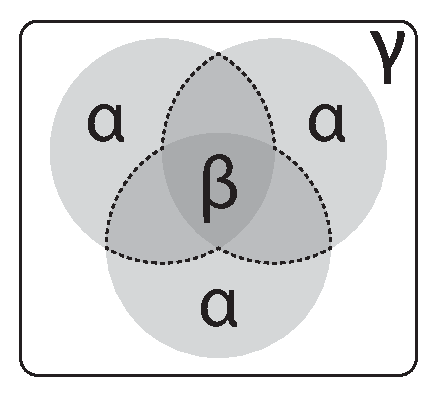
\includegraphics[width=0.7\textwidth]{./figures/Introduction/diversities}
  	\caption{Schematic representation of $\alpha$ (gray circles), $\beta$ (dotted line) and $gamma$ (blach square) diversities.\label{fig:diversities}}
\end{figure}
These indices are linked to the area of interest which can be of different sizes and, the habitats or the sites within it may vary their dimensions, accordingly. Both $\alpha$ and $\gamma$ diversities are subjected to the spatial scale chosen but no consensus has been reached on what spatial scales are appropriate to quantify these indices \cite{whittaker2001scale}. Therefore, it has been proposed that the definition of $\alpha$ and $\gamma$ diversities does not need to refer to a specific spatial scale: these indices can be measured for an existing environment of any size that consists of subunits at any scale. These scale-free definition is not applicable to $\beta$-diversity as it can not be calculated directly from a species data \cite{tuomisto2010diversity}. Beta diversity in his original definition has to be considered as a measure of the species turnover between two sites \cite{whittaker1960vegetation}. The simplest definition of this index is: $\beta = \gamma/\alpha$; where gamma diversity is the total species diversity of a landscape, and alpha diversity is the mean species diversity per habitat. Here $\beta$-diversity quantifies how many subunits there would be if the total species diversity of the whole environment and the mean species diversity per sites remained the same, but the latter shared no species. Given these definitions of diversity measures, studying microbial populations in a particular environment requires the collection of ``samples'' able to inform us about the real natural diversity of that environment, but how can we estimate diversity?\\
Several diversity indices have been used by researchers to quantify diversity, each one with its own characteristics and limits. One of the simplest diversity index is the so-called \textbf{species Richness} (usually noted, and here referred, as $S$), that is the number of different species detected in a given community. Although it gives a measure of the biodiversity of a particular environment, this index does not take into account any distribution parameter (like the relative abundance distribution of the species). In order to have a more detailed perspective of the biodiversity of a site others more complex indices have been developed considering species abundance data and probabilistic functions.
\subsubsection*{True diversity}
\label{sec:tdiversity}
This value is a measure of the effective number of types (or species); it refers to the number of equally-abundant types needed for the average proportional abundance of the types to equal that observed in the dataset of interest (where all types may not be equally abundant). The true diversity in a dataset is calculated by first taking the weighted generalized mean of the proportional abundances of the types in the dataset, and then taking the inverse of this \cite{tuomisto2010diversity}:
\begin{equation*}
{}^q\!D={1 \over \sqrt[q-1]{{\sum_{i=1}^S p_i p_i^{q-1}}}}
\end{equation*}
Here $p_i$ represent the proportional abundance of the $i$-th species, whereas $q$ is a ``sensitivity'' parameter that defines which kind of mean is used. With a sensitivity of 0 the mean corresponds to the weighted harmonic mean, which is 1/S because the $p_i$ values are removed. For a value of $q$ equal to 1 this equation is undefined and for a value equal to 2 the equation corresponds to the arithmetic mean. On the contrary, for increasing values of $q$ the generalized mean approaches the maximum $p_i$ value. In other words, $q$ modifies species weighting, such that increasing $q$ increases the weight given to the most abundant species. Consequently, for the same dataset,it is possible to obtain larger or smaller values of species diversity increasing or decreasing $q$, respectively. In case that all species are equally abundant, the value of $q$ has no effect on the diversity computation, which will be equal to the richness for every value of $q$.\\
\subsubsection*{Shannon-Wiener function}
The Shannon-Wiener function is one of the most popular diversity index used in Biology and Ecology even if its first definition was proposed independently by Claude Shannon and Norbert Wiener to quantify the entropy (uncertainty or information content) in strings of text \citep{shannon1949mathematical, wiener1948cybernetics}. It has been called with a variety of names from Shannon-Weaver index (where Weaver refers to Wallace Weaver, Shannon's co-author) to Shannon entropy, but its correct definition is Shannon-Wiener function as reported in \citep{krebsj}. This index is based on the idea that more different species there are in a sample, and the more equal their proportional abundances are, the more difficult is to correctly predict the next randomly chosen species from the sample. It is most often calculated as follows:
\begin{equation*}
H' = -\sum_{i=1}^S p_i \ln p_i
\end{equation*}
let $p_i$ be the proportional abundance of the $i$-th species; this formula quantifies the uncertainty in predicting the species identity of an individual that is taken at random from the dataset. Historically, this equation is written using the natural logarithm, but it can be written freely choosing the base of the logarithm. Nevertheless, the most popular logarithmic bases are 2, 10 and e, corresponding to three different measurement units, which have been called binary digits (bits), decimal digits (decits) and natural digits (nats), respectively. Before comparing values of this index obtained with different logarithmic bases, it is required to convert them to the same logarithmic base and this can be done, as reported in Shannon work, multiplying one base for the log of the other base (for example if we want to change from the base $a$ to base $b$, this can be obtained with multiplication by $\log_{b}a$).\\
When all species found in a site of interest are equally common, all $p_i$ values equal $1/S$, and the Shannon-Wiener function hence takes the value $ln S$. The more unequal the abundances of the species, the smaller the corresponding Shannon entropy. Practically, if one species is very abundant, and the others are extremely rare (even if there are many of them), Shannon entropy approaches zero. In particular, if one site contains only one species, Shannon entropy exactly equals zero (in other words, there is no uncertainty in predicting the type of the next randomly chosen entity).\\
Another index similar to the Shannon-Wiener function is the \textbf{R\'{e}nyi entropy} \cite{alfred1960measures}. This index takes into account the same sensitivity parameter $q$ explained above in the~\nameref{sec:tdiversity}~section. In particular, the R\'{e}nyi entropy is a generalization of the Shannon entropy to other values of $q$ than unity, and it can be expressed as:
\begin{equation*}
{}^qH = \frac{1}{1-q} \; \ln\left ( \sum_{i=1}^R p_i^q \right )
\end{equation*}
This expression can be written in another format:
\begin{equation*}
{}^qH = \ln\left ( {1 \over \sqrt[q-1]{{\sum_{i=1}^R p_i p_i^{q-1}}}} \right )
\end{equation*}
that is (see~\nameref{sec:tdiversity}~section): 
\begin{equation*}
\ln({}^q\!D)
\end{equation*}
\subsubsection*{Simpson index}
This index was introduced for the first time by Edward H. Simpson in 1949 \cite{simpson1949measurement} for measuring the degree of concentration when individuals are classified into types. In Biology and Ecology this index is used to quantify the probability that two entities taken at random from the dataset of interest represent the same type. It is computed using the following formula: 
\begin{equation*}
\lambda = \sum_{i=1}^S p_i^2
\end{equation*}
In its original definition this index is more a measure of equality than diversity; in fact, the higher the value of this index, the smaller the number of different species in the dataset. Proportional abundances ($p_i$) are by definition constrained to values between zero and one, but their weighted arithmetic mean, and hence the Simpson index, can never be smaller than 1/S, which is reached when all types are equally abundant. As said before, since mean proportional abundance of the types increases with decreasing number of types and increasing abundance of the most abundant type, this index assumes small values in sites with high diversity and,
contrariwise, large values in sites with low diversity. This can be a counter-intuitive behaviour for a measure of diversity, so transformations of $\lambda$ that increase with increasing diversity have been often used. Two of the most popular of such transformations are the \textbf{inverse Simpson index} (defined as $1/\lambda$) and the \textbf{Gini–Simpson index} (defined as $1 - \lambda$) \cite{hill1973diversity,jost2006entropy}. It is worth noticing that both of these modification of the original Simpson index have been used in literature, usually referring to them as Simpson index, so care is needed to avoid accidentally comparing the different indices as if they were the same.\\
\bigskip

Despite the high number of diversity indices and their different characteristics, all biologists who sample natural communities are plagued with the problem of how well a sample reflects a community's ``real'' diversity. Ecologists studying the diversity of macroorganisms have faced this estimation problem and have designed tools for dealing with the problem of sampling \cite{heck1975explicit, magurran1988ecological, colwell1994estimating}. The availability of microbial diversity data have increased the interest in applying these ``ecological'' tools to the microbial world. Several microbial studies have used diversity indices for comparing sample diversity, but their suitability is not completely clear \cite{mcmurdie2014waste}. Others new diversity estimators have been proposed in order to deal with microbiological data. However, the success of these tools has not yet been fully evaluated for microbial communities, and other approaches remains to be explored.\\
Estimating microbial diversity is not a trivial task and finding a way to compare how well this diversity has been estimated can be even harder. One possible way to face this problem is based on the assumption that in any community, the number the number of organism types detected increasing with sampling effort until all types are detected. The relation between the number of observed types and the sampling effort can be used as a possible measure of the total diversity of the sampled community. An accumulation curve is a possible way to inspect this relation simply plotting the cumulative number of types observed versus the sampling effort (as number of sampled units); in this way, differences in ``species diversity'' of the sampled community underlie differences in the shape of the curve. If the sampling effort is pushed to its maximum, the curve would eventually reach an asymptote representing the ``real'' number of different types in the observed community. In other words, the more concave-downward the curve, the better sampled the community. Another possible way to compare how well communities have been sampled is to plot their rank-abundance curves. In this plot, species are ordered from the most to least abundant on the $x$ axis; whereas the abundance of each observed species is plotted on the $y$ axis. Sample containing high number of rare species will produce a long right-hand tail, whereas samples with an equal proportional abundance of species will produce an almost squared plot.\\



%%-----------
%% Backmatter
%%-----------
\backmatter
\chaptermark{Bibliography}
\renewcommand{\sectionmark}[1]{\markright{#1}}
\bibliographystyle{unsrt}                           %Use alpha codes for references
\sectionmark{Bibliography}
\addcontentsline{toc}{chapter}{Bibliography}        %Force addition of Bibliography to TOC    
\bibliography{References}